\chapter{Multimodal Black-box Models}
\label{chapter:multiodality}

\textit{"Learning is lifelong; we forget rules when they no longer apply or revise them when the environment changes."} - Ethem Alpaydin, Machine Learning: The New AI 

\section{Chapter Overview}
In the previous chapter, we used only CNVs, i.e., single modality to develop a decision support system~(DSS), which was technically a black-box model based on snapshot neural ensemble method in which we trained two deep architectures called \texttt{Conv-LSTM} and \texttt{CAE}. The DSS moderately performed at predicting cancer types. However, our real world experience is multimodal~\cite{mmsurvey}, e.g., while watching a movie, we not only observe the movie itself but the acting, background music, action, background scenario, and landscapes, etc. Multimodal machine learning~(ML) aims to build a ML model capable of processing and relating information from multiple modalities~\cite{mmsurvey}. Concerning our cancer CDSS, multiple factors are involved~(e.g., in cancer diagnosis, estrogen receptor~(ER), progesterone receptor~(PGR), and human epidermal growth factor receptor 2~(HER2/neu statuses for breast cancer), providing AI-based diagnoses might not be accurate solely based on CNVs. This requires using multimodal features based on DNA methylation, gene expression, miRNA expression, and CNVs data by creating a multiplatform network to support each data type, where the DSS based on CNV data along with other types of genomics data from different cohorts such as DNA methylation, gene expression, and somatic mutations will be more reliable. 

\hspace*{3.5mm} Based on this motivation, in this chapter, we extend the single modality to multimodality-based cancer typing method by employing a multimodal neural network approach to analyze genomics data from TCGA to classify breast cancer patients based on their subtypes. We hypothesize\footnote{\textbf{H3}: Multimodal genomics data and clinical outcome can be used to train a multimodal neural network architecture to provide more accurate clinical diagnostic decision.} that multimodal genomics data and clinical outcome can be used to train a multimodal neural network architecture to provide more accurate clinical diagnostic decision.
%and survival rates. 
In particular, we used DNA methylation, gene expression~(GE), and miRNA expression data by creating a multiplatform network called multimodal autoencoders~(MAE) classifier to support each data type\footnote{RQ1: How to use multimodal genomic data to accurately predict cancer
types?}. We will observe the effect of different modalities and assess the performance of our CDSS across breast cancer subtype classification. 
%Experiment results demonstrate that our approach is promising with high confidence for predicting both breast cancer subtypes and survival rates. In particular, we achieved state-of-the-art results with accuracies of $91\%$ and $86\%$, respectively for the ER and PGR-based subtype prediction and moderately low accuracy for the HER2-based subtype prediction as well as we perceived reasonably low MSE and positive coefficient of determination~($R^2$) scores in case of survival prediction. 
%Additionally, we created unimodal and multimodal features from each input type and trained decision tree~(DT), Naive Bayes~(NB), K-nearest neighbors~(KNN), logistic regression~(LR), support vector machine~(SVM), random forest~(RF), and gradient boosting trees~(GBT) as ML baseline models. We use the model averaging Ensembl of top-3 models to report the final prediction based on how the clinical DSS recommends decision. Further, we provide in details analysis of the MAE model. 

\section{Introduction}
\label{secIntroduction_Motivation}
Multimodal information fusion seeks to improve the performance of a DSS (based on an inference model) by efficiently combining useful information extracted from a set of distinctive modalities~\cite{mmdcae}. The performance of a conventional information fusion architecture is greatly affected by its ability to detect and combine useful and complementary information from heterogeneous representations stemming from a set of distinctive modalities~\cite{ito2018effects}. Multimodal fusion is the concept of integrating information from multiple modalities with the goal of predicting an outcome measure~\cite{mmsurvey,mmdcae}. Multimodal fusion provides three main benefits~\cite{mmsurvey}: i) having access to multiple modalities that observe the same phenomenon may allow for more robust predictions, making the clinical DSS more reliable, ii) having access to multiple modalities might allow us to capture complementary information, e.g., we can often integrate genomics, proteomics, bioimaging, texts, or even clinical outcomes to support each other, iii) a multimodal system can still operate when one of the modalities is missing, e.g., in case of missing bioimaging, we can still rely on genomics, proteomics, and clinical outcomes.

\hspace*{3.5mm} Concerning to the cancer DSS, accurate diagnosis and prognosis to cancer are specific to patients with particular cancer subtypes and molecular traits e.g. accurate treatments for the breast cancer patients depends on several distinct molecular subtypes such as `Luminal A', `Luminal B', `HER2-enriched', and `Triple-negative'~(TN)~\cite{sorlie,dai}, which subject to the distinction mainly determined by several factors: `Luminal A' disease generally requires only endocrine therapy, chemotherapy is considered necessary for `Luminal B', `HER2-enriched', and `Triple-negative' patients~\cite{goldhirsch}. Thus, knowing the subtypes of any breast cancer patient is essential before recommending the best possible treatment. 
TN breast cancer defined by ER, PGR, and HER2, represents a subset of breast cancer with different biologic behavior. ER, PGR, and HER2 statuses are mainly involved in determining breast cancer subtypes. %and survival rates. 
Further, those patients can be categorized into different classes. For example, ER `POSITIVE', `NEGATIVE', or `INDETERMINATE'. The ER-negative tumors are associated with a worse clinical outcome compared to ER-positive disease. An accurate estimate of the hazard ratio between ER-negative tumors and ER-positive tumors remains difficult and prone to higher misclassification~\cite{karimACCA2019}. 
%As cancer is a disease that was caused by genetic mutations, more extensive knowledge of each mutation might result in the further distinction of breast cancer subtypes.
%The survival rate, on the other hand, suggests the chance of survival based on patients clinical and pathology information, which are further dependent on the in-depth analysis of these status biomarkers. %An analysis of genetic mutations directly on the survival rate data might tell the whole picture of why some genetic mutations might cause the worst cancer than other mutations.

\hspace*{3.5mm} In order to develop a more robust and efficient DSS, it needs to be able to interpret such multimodal perspectives together~\cite{mmsurvey}. However, multiple modes of information are gathered to create knowledge in a way humans can understand~\cite{mmdcae}. However, each type of data has different intrinsic statistical features that cannot be compared in a trivial way, nor they can be combined. In this chapter, we develop a clinical DSS using DNA methylation, GE, and miRNA expression data in a single analysis by creating an MAE to handle the shared representation of the multiplatform data to support each other. We hypothesize\footnote{    \textbf{$H_2$}: neural representation learning can be more effective for learning high-level abstract features against data sparsity.} that neural representation learning can be more effective for learning high-level abstract and multimodal features against data sparsity. 
The rest of the chapter is structured as follows: \cref{chapter_4:rw} covers related works concerning cancer diagnosis based on multimodality data and summarize their potential limitations. \Cref{chapter_4:mm} describes the overall approach, including the detail of the data collection and feature engineering before the network construction and training. \Cref{chapter_4:results} demonstrates the experiment results. \Cref{chapter_4:discussion}, discusses key findings of the study. \Cref{chapter_4:conclusion} provides some explanations of the importance and relevance of the study reported, highlights the limitations and discuss some future works before concluding the chapter. 

\section{Related Work}\label{chapter_4:rw}
The multilayer nature of DNN's each successive layer is hypothesized to represent the data in a more abstract way~\cite{mmsurvey}. Hence it is common to use the final or penultimate neural layers as a form of data representation~\cite{mmsurvey,serban2016multi}. To construct a multimodal representation using neural networks each modality starts with several individual neural layers followed by a hidden layer that projects the modalities into a joint space~\cite{serban2016multi}. The joint multimodal representation is then be passed through multiple hidden layers itself or used directly for prediction. Such models can be trained end-to-end-learning both to represent the data and to perform a particular task, e.g., classification. This results in a close relationship between multimodal representation learning and multimodal fusion when using DNN~\cite{wang2018associativemulti}.

\hspace*{3.5mm} The model proposed by Ngiam et al.~\cite{NgiamKKNLN11} extended the idea of using autoencoders to the multimodal domain. They used stacked denoising autoencoders to represent each modality individually and then fused them into a multimodal representation using another autoencoder layer~\cite{mmsurvey,serban2016multi}. It is also common to fine-tune the resulting representation on a supervised learning tasks such as regression or classification. The major advantage of DNN-based joint representations comes from their often superior performance and the ability to pre-train the representations in an unsupervised manner. The performance gain is, however, dependent on the amount of data available for training. One of the disadvantages comes from the model not being able to handle missing data, which is mainly due to the reconstruction losses during the pre-training goes unbound. Usually, a DNN require a lot of labeled training data. Therefore, it is common to pre-train such representations using an autoencoder on unsupervised data~\cite{mmsurvey}. 

\hspace*{3.5mm} Even a few years ago, most popular approaches for graphical-model based representation are deep Boltzmann machines~(DBM), that stack restricted Boltzmann machines~(RBM) as building blocks. Similar to DNNs, each successive layer of a DBM is expected to represent the data at a higher level of abstraction. The appeal of DBMs comes from the fact that they do not need supervised data for training. As they are graphical models the representation of data is probabilistic, however it is possible to convert them to a deterministic DNNs, which, however, loses the generative aspect of the model. Although, approaches using both unimodal~\cite{abdel2016breast} and multimodal DBN~\cite{liang} show accuracy at different prediction tasks, one of the potential limitations using DBN-based approaches is that the limited capability at feature learning during pretraining~\cite{serban2016multi}, although it gets a decent set of feature representations for the inputs. Furthermore, DBN is incapable of learning quality features from very high dimensional datasets. Besides, pretraining losses often get out of bound, which results in overfitting issue. 

\hspace*{3.5mm} To overcome these limitations, majority of the multimodal methods focused on representation fusions~\cite{ito2018effects}, either by combining representations before the classification called feature level fusion or by combining the results of classifications performed in single-mode representations in another analysis  called `decision level fusion'~\cite{atrey2010multimodal}. In particular, researches have proposed multimodal autoencoder~(MAE)-based approaches~\cite{liu2016multimodal,serban2016multi,wang2018associativemulti}, which is a flexible, simple prior distribution which can be learned efficiently and potentially capture from extensive features of a target distribution. Consequently, MAE has shown tremendous success in natural language understanding tasks like document modeling and dialogue modeling~\cite{serban2016multi}, in computer vision like emotion recognition~\cite{liu2016multimodal}, and multimodal word representation~\cite{wang2018associativemulti}. 

\hspace*{3.5mm} An alternative to a joint multimodal representation is a coordinated representation, where instead of projecting the modalities together into a joint space, separate representations for each modality are learned but coordinated them through a constraint. Inspired by these successes, we construct a MAE network by extending the multimodal system presented in~\cite{wang2018associativemulti} by adding the capability of handling multiple modalities across four different types of genomics data. Then we added a fully connected layer for the supervised learning task, i.e. breast cancer subtypes predictions. However, our datasets are very rich, covering all the modalities for $93\%$ of patients. In our approach, we apply multimodal fusion approach by discarding the small part of patient data that don't have all modalities in our MAE network. Although, there a few recent multimodal approaches for more optimized representation learning, in this chapter we will observe the performance of vanilla autoencoder-based MAE architecture. 

\section{Methods}\label{chapter_4:mm}
In this section, we discuss our approach in detail, including data collection, preprocessing, network construction, and training. 
%\subsection{Problem statement}
%Although breast cancer patients now have one of the best survival rates among other cancer types, improved studies on breast cancer are still a non-trivial research problem. 
%We focus here on the difficult problem of finding sub types of breast cancers. 
Since we conceive finding the importance of extensive knowledge about genetic mutations in breast cancer aiming to help in discovering more suitable treatments for each breast cancer subtypes, we show which genetic mutations are responsible for which breast cancer subtypes~(with feature selection). % or have direct correlations on the survival rates.  %, which is because certain genetic mutations might have a direct correlation on survival rates. %To summarize, the following tasks will be completed:
For the breast cancer subtypes prediction, we used genomics data accompanied by ER, PGR, and HER2/neu status that are present inside breast cancer patients for each patient either separately or in a multimodal way. We adaptively capture the heterogeneity of expression across samples in a gene regulation space, instead gene expression space. The idea is to transform gene/miRNA expression and DNA methylation profiles into regulation profiles for characterizing differential expression of genes between different subtypes for breast cancer.
%In the context of survival rate prediction, our network should tell us the chance of survival for each cancer patient based on individual patient's clinical and pathology information. The survival rate ranges between [0-1], with 1 being the highest chance of survival.
%Since data is essential for training the MAE model, 
%We provide the details of the data collection, processing, and feature selection in details. 

\begin{sidewaysfigure*}
	\centering
	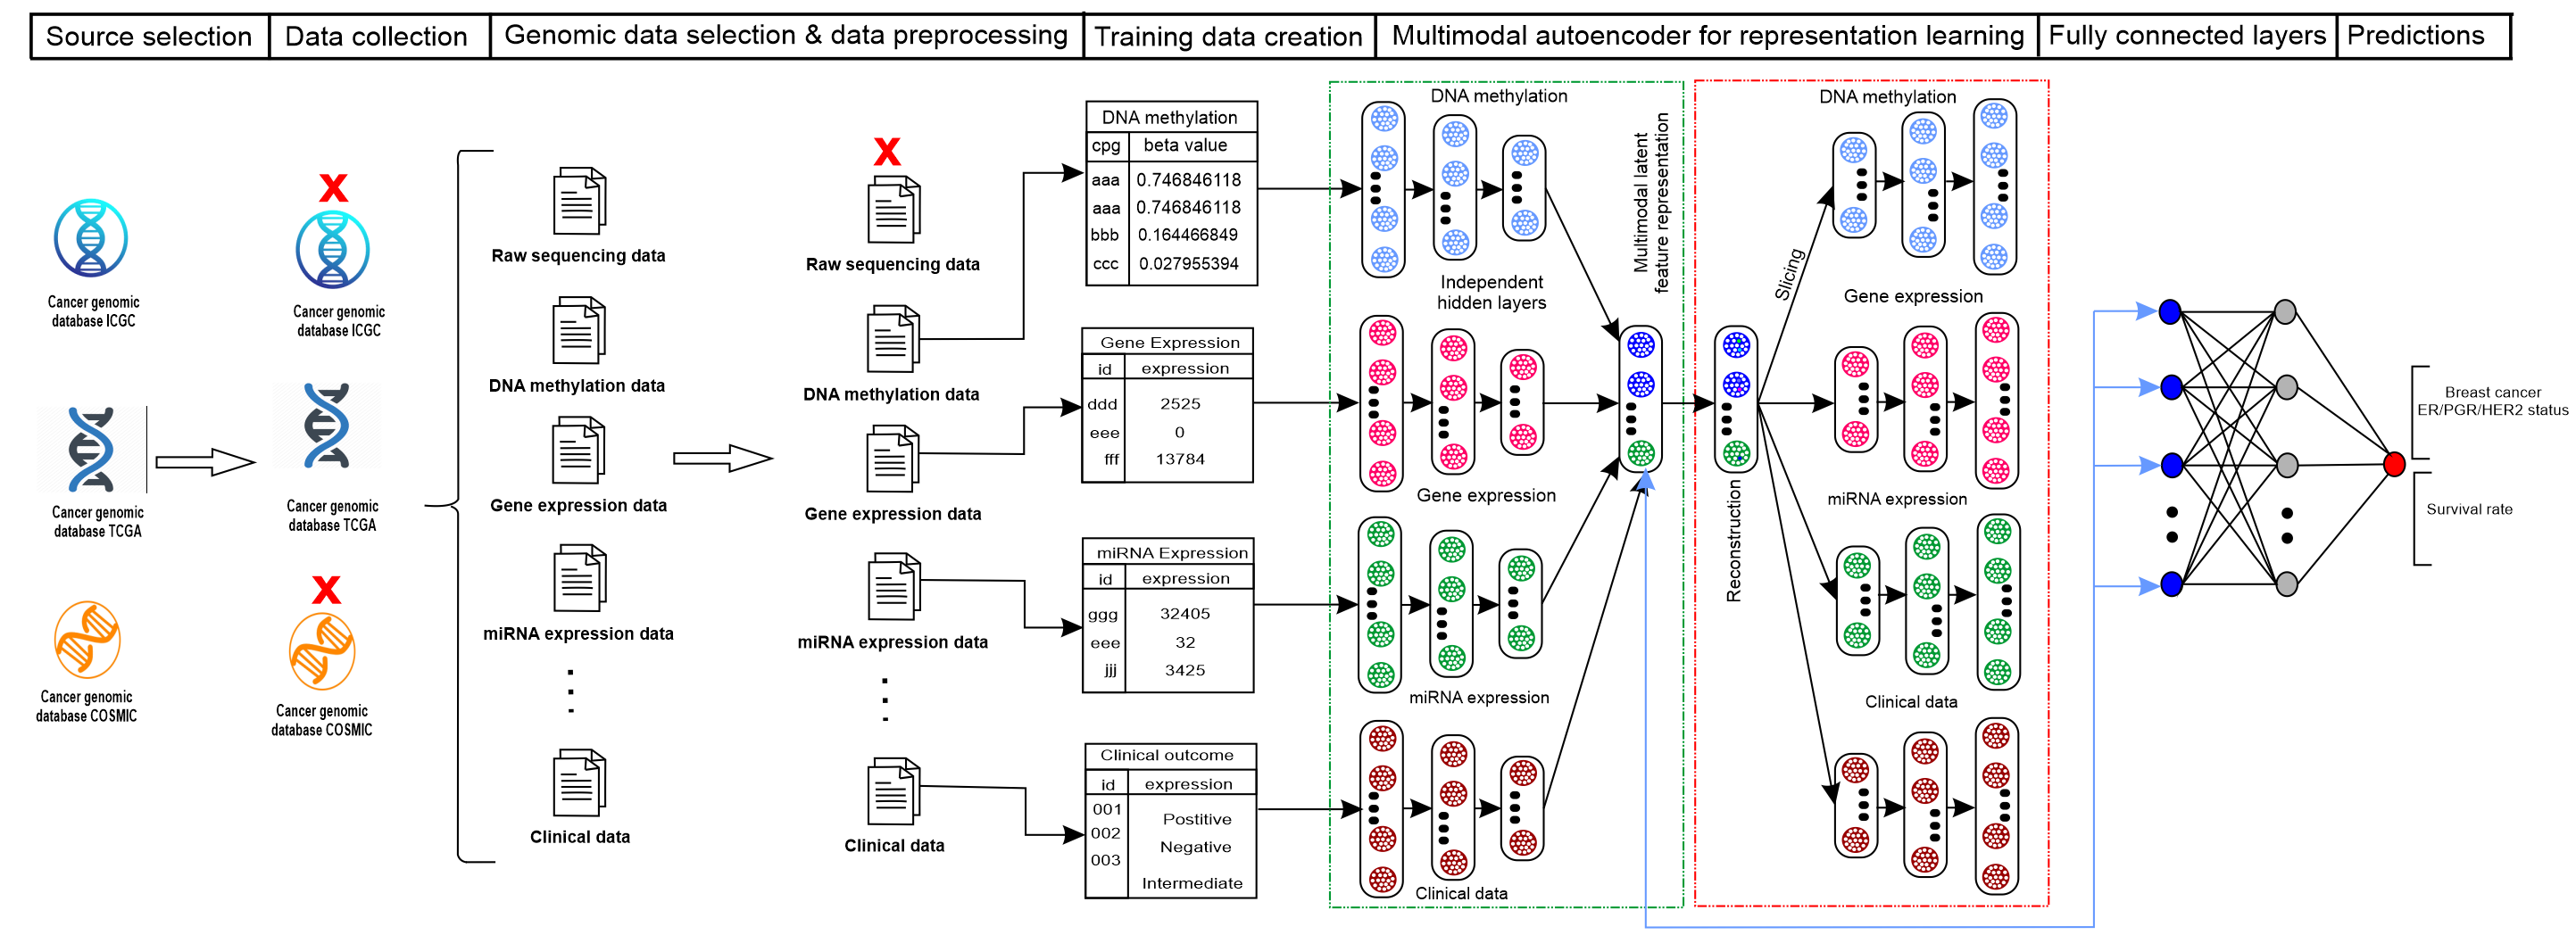
\includegraphics[width=\textwidth]{images/mae_v2.png}
	\caption{Workflow of the proposed approach in which same input types with different features for subtypes %and survivals 
	are used~\cite{karimACCESS2019}.}
	\label{fig:wf_mae}
\end{sidewaysfigure*}

\subsection{Datasets and feature selection}
\label{dc}
Although genomics data covers all data related to DNA on living organisms, we use transcriptomics data, including RNA and miRNA. These genomics data are usually accompanied by clinical outcomes, which comprise of general clinical information as well as cancer status (e.g., cancer location, cancer stage). These data are also very high-dimensional, e.g., GE data for each patient, which is structured based on gene id reaches around 60,000 types, meaning a predictor based on GE comes with 60,000 different features. Several databases of genomics data exist including TCGA~\cite{tcga}, ICGC~\cite{icgc}, and COSMIC~\cite{forbes}. However, based on public availability and amount of data consideration, e.g., the number of patients data and clinical outcomes, we considered the breast invasive carcinoma~(BRCA) branch of TCGA as the main source of data\footnote{TCGA has 39 projects for 39 different cancer types~(v89)}. After selecting data sources, we start collecting both clinical data and biospecimens through the Genomics Data Commons~(GDC) data portal\footnote{\url{https://portal.gdc.cancer.gov/}}. 

\hspace*{3.5mm} To provide more reliable cancer identification 
%and the decision about survival
, several modalities consisting of masked somatic mutations, copy number segment~(CNS) and mask CNS, DNA methylation, GE, miRNA expression along with clinical outcomes were used, instead of a single modality. Besides, some preprocessed data were reused\footnote{Based on a Master thesis I co-supervised with Dr. Oya Beyan: "Analysis of Breast Cancer Genomic Data with Multimodal Deep Belief Network", by Galih Wicaksono, Software Systems Engineering, RWTH Aachen University, 2018.}. Some of the data comes in different formats, e.g., $70\%$ of the DNA methylation data of breast cancer patient came from a different platform than the remaining $30\%$, having two structures. 

\begin{table}[h]
    \scriptsize
    \caption{Statistics of the data used for breast cancer sub-typing~\cite{karimACCESS2019}}
    	\vspace{-2mm}
    \label{tab:all_data_brca}
    \centering
    \begin{tabular}{l|l|l|l} 

        \hline
        \textbf{Tasks}   & \textbf{Input modality} & \textbf{\#Sample } & \textbf{\#Features}  \\ 
        \hline
             & DNA methylation  & 1,046  & 25,978  \\ 
        \cline{2-4}
               & Gene expression   & 1,042 & 60,483      \\ 
        \cline{2-4}
        ER status classification       & miRNA expression                           & 1,029                & 1,881       \\ 
        \cline{2-4}
                                       & Gene + miRNA expression                   & 1,024                & 62,364      \\ 
        \cline{2-4}
                                       & Gene + miRNA expression + DNA methylation & 1,022                & 88,342      \\ 
        \hline
                                       & DNA methylation                           & 1,045                & 25,978      \\ 
        \cline{2-4}
                                       & Gene expression                           & 1,041                & 60,483      \\ 
        \cline{2-4}
        PGR status classification      & miRNA expression                           & 1,028                & 1,881       \\ 
        \cline{2-4}
                                       & Gene + miRNA expression                   & 1,023                & 62,364      \\ 
        \cline{2-4}
                                       & Gene + miRNA expression + DNA methylation & 1,021                & 88,342      \\ 
        \hline
                                       & DNA methylation                           & 917                  & 25,978      \\ 
        \cline{2-4}
                                       & Gene expression                           & 913                  & 60,483      \\ 
        \cline{2-4}
        HER2/neu status classification & miRNA expression                           & 902                  & 1,881       \\ 
        \cline{2-4}
                                       & Gene + miRNA expression                   & 897                  & 62,364      \\ 
        \cline{2-4}
                                       & Gene + miRNA expression + DNA methylation & 895                  & 88,342      \\ 
        \hline
        \iffalse
                                       & DNA methylation                           & 1,082                & 25,978      \\ 
        \cline{2-4}
                                       & Gene expression                           & 1,077                & 60,483      \\ 
        \cline{2-4}
        
        Survival prediction            & miRNA expression                           & 1,064                & 1,881       \\ 
        \cline{2-4}
                                       & Gene + miRNA expression                   & 1,058                & 62,364      \\ 
        \cline{2-4}
                                       & Gene + miRNA expression + DNA methylation & 1,056                & 88,342      \\ 
        \hline
        \multicolumn{1}{l}{}           & \multicolumn{1}{l}{}                      & \multicolumn{1}{l}{} &  
        \fi 
    \end{tabular}
    	\vspace{-4mm}
\end{table}

\hspace*{3.5mm} However, in our case, several factors refrained us from using each type of data, e.g. masked somatic mutation data are the base pair~(BP) position in a chromosome but 
%The total number of base pairs in a single human cell 3 billion and 
not all the mutations are significant. Even if we use them, the generated dataset will be very sparse. %giving too many zero entries. 
The CNS and masked CNS data were not used because of extremely high dimension and complex structure of the data, and there was no fixed dimension for each data per patient. Since BP's start refers observed, CNS data and stop positions in a chromosome, which will always vary at a BP resolution.
%We do not use here copy number and DNA variation gave the extremely high dimension and complex structure of the data, i.e., variant position, will always vary at a base pair resolution.
With these considerations, DNA methylation, GE, and miRNA expression data along with clinical data containing pathology response data are used. 
%and the survival rate data are used.
Since the GE quantification data covers the amount of RNA synthesized by each gene on a single time, we treat each data per row and consider if the gene's Ensembl Id belongs to the Ensembl Id Release 89. The miRNA expression quantification and GE quantification data from TCGA were already in the desired format, so no preprocessing was required. 
%From the masked somatic data, gene data containing both the Ensembl ID and Hugo gene symbol considered only. Since both CNS and masked CNS data cover entire gene mutation cases on base-pair sequences instead of a single BP case, which was covered in masked somatic data, we find corresponding Ensembl gene ID from the chromosome position and extract the data using Ensembl API~\cite{yates}. 

\hspace*{3.5mm} However, processing DNA methylation data was a complex task as some patients were measured with the HumanMethylation27 platform. The remaining patients were measured with HumanMethylation450 arrays, which measures 450.000 methylation sites, being only 26K DNA methylation sites were considered in common to both platforms. We combined these data in seven modalities:~DNA methylation, GE, miRNA expression, GE+miRNA expression, DNA methylation+GE+miRNA expression, GE+DNA methylation, and miRNA expression+DNA methylation within the data\footnote{Last two modalities were used for the training and evaluation but not reported due to low accuracies.}. \Cref{tab:all_data_brca} shows the statistics of the preprocessed data for each modality. We find corresponding Ensembl gene IDs from the chromosome position based on GDC API. The samples having the latest gene Ensembl IDs from Release 89 are only considered valid. Clinical data covers clinical outcomes of cancer patient treated as general, pathology, treatments, and surgery. We categorized each patient data into different groups, but only the pathology response 
%and the survival data 
from the whole clinical outcomes are used. 

%\subsection{Selection of neural networks}
%We restrict our selection on DNN architecture based on the types of data: since we don't have enough labeled data, using CNN was not a viable option at first place because an end-to-end CNN requires huge data to get trained well. Secondly, since the data at our hand is not in sequence format (e.g., raw DNA sequence or protein sequence), we decided not to use RNN types networks. 
%Thirdly, the multimodality nature of the input data further motivated us developing a deep multimodal architecture called Multimodal Autoencoders~(MAE).% input which includes different type of data (e.g., audio and video), which was first proposed by Ngiam et al\cite{NgiamKKNLN11}. 

\subsection{Network construction and training}
The multimodality nature of the input data further motivated us developing the MAE. Although a single and simple AE discussed in \cref{preli:AEs} can reconstruct an output similar to the original input, it cannot handle multimodality~(i.e., different types of information). Nevertheless, traditional supervised learning is only able to learn from the intersection of samples, which are both clean and labeled. In contrast, the weights of the MAE encoder learn from both clean, unsupervised data with no labels, and noisy supervised data with missing modalities, leveraging as much of the available data as possible. Architecturally, MAE is similar to a three-stage AE: the first stage represents a particular modality for each type of data, and the second stage represents the cross-modality. The AE is used to find a low-dimensional representation of multimodal data, taking advantage of the information that one modality provides about another. We illustrate the construction of an MAE as a quad-modal AE for this problem. Where DNA methylation, GE, miRNA expression, and clinical outcomes form four different modalities. 

\hspace*{3.5mm} The individual modality AE is not only a one-layer AE, but a multilayer and gradually shrinking AE with the possibilities of a different number of layers for each modality, which is due to the difference in dimension between modalities are pretty large, e.g. GE data consists of around 60,000 features, while miRNA data only consists of around 1,800. By default, the AE network fusing multiple modalities consists of a variable number of ReLU layers, which are densely connected. The cross-modality AE is also a multilayer gradually shrinking AE with different size of output layer for each prediction. However, the number of layers and number of units per layer of the encoder and decoder networks are symmetric. The third stage is the supervised MAE in which the decoder part is removed, and only the encoder part is utilized by adding a fully connected layer. % for the classification. %and regression operations. 
First, data $X_{i,j} \in \mathbb{R}^{D}$, for each modality $i \in \mathbb{N}$\footnote{N represents the dimensionality of the $i^{th}$ input modality} is fed into the encoder $f_{\theta_{i}}$ in order to generate a modality specific latent representation $h_{i, j}$ as follows~\cite{mmdcae}: 

\vspace{-4mm}
\begin{align}
    h_{i, j}=f_{\theta_{i}}\left({X}_{i, j}\right)
\end{align}

where $f_\theta$ signifies trainable parameters of the encoder specific to the $i^{th}$ modality. Subsequently, the latent representation is then fed into the decoder module to reconstruct ${X}_{i, j}^{\prime}$ similar to the original input. The parameters of the modality specific AE are then then trained to minimize the RL1 between the decoder’s output and the input signal, where the RL1 is similar \cref{eq:Loss1}. The latent representations of all modalities are further concatenated into a single representation $h_{i,j} \in \mathbb{R}^{D}$. 

\hspace*{3.5mm} However, in order to create such a shared representation, it is required that all latent representations have the same dimensionality such that $\forall i \in\{0,1, \ldots, n\}, d_{i}=$ $\eta \in \mathbb{N}$~\cite{mmdcae}. On the other hand, the architecture depicted in \cref{fig:slr_1} generates the shared representation for all input modalities, instead of one latent representation for each input modality. However, for the simplicity, in this chapter, we use the shared representation for all input modalities. In either approach, the resulting concatenated generates a single vector $u=\left[u_{0}, u_{1}, \ldots, u_{n}\right] \in[-1,1]^{(n+1) \eta}$, where the weights of the corresponding components are generated using the softmax layer as follows~\cite{mmdcae}:

\vspace{-6mm}
\begin{align}
    \omega=\operatorname{softmax}\left(W_{\omega} u+b_{\omega}\right),
\end{align}

where $\omega=\left[\omega_{0}, \omega_{1}, \ldots, \omega_{n}\right] \in[0,1]^{(n+1) \eta}$ $\left(\forall i, \omega_{i} \in[0,1]^{\eta}\right)$, and  $W_{\omega} \in$
$\mathbb{R}^{(n+1) \eta \times(n+1) \eta}$ and $b_{\omega} \in \mathbb{R}^{(n+1) \eta}$ is the trainable parameters ~\cite{mmdcae}. The final latent representation is generated through a weighted sum of all the modalities specific latent representation $\left(h_{i,j}\right)$ based on the computed weights $\left(\omega_{i}\right)$ as follows~\cite{mmdcae}: 

\vspace{-4mm}
\begin{align}
   h_{i,j}=\sum_{i=1}^{n}\left(h_{i} \odot \omega_{i}\right),
\end{align}

where $\odot$ denotes the element-wise product and $h \in$ $\mathbb{R}^{\eta}$ is the final representation~~\cite{mmdcae}, which is subsequently fed to the classifier for the classification. In our approach, as shown in ~\cref{fig:wf_mae}, our model first transforms input DNA methylation vector $x_m$, GE vector $x_e$, miRNA expression vector $x_r$, and clinical data vector $x_c$ to hidden representations~\cite{wang2018associativemulti}.

\vspace{-4mm}
\begin{align}
    \begin{array}{l}
        {h_{m}=g\left(W_{m} x_{t}+b_{m}\right)} \\
        {h_{e}=g\left(W_{e} x_{v}+b_{e}\right)} \\
        {h_{r}=g\left(W_{r} x_{a}+b_{r}\right)} \\
        {h_{c}=g\left(W_{c} x_{t}+b_{c}\right)}
    \end{array}
    \label{eq:m1}
\end{align}  

Then the hidden representations are concatenated together and mapped to a common space~\cite{liu2016multimodal}:

\vspace{-4mm}
\begin{equation}
    h_{mae}=g\left(W_{mme}\left[h_{m} ; h_{e} ; h_{r} ; h_{c}\right]+b_{mme}\right)
\end{equation}

The model is trained to reconstruct the hidden representations of the three modalities $h_{mae}$:

\vspace{-4mm}
\begin{equation}
    \left[\hat{h}_{m} ; \hat{h}_{e} ; \hat{h}_{r} ; \hat{h}_{c} \right]=g\left(W_{mae}^{\prime} h_{mae}+b_{\hat{mae}}\right)
\end{equation}

To reconstruct the original representation of different modalities i.e., DNA methylation, gene expression, miRNA expression data, and clinical outputs~\cite{wang2018associativemulti}: 

\vspace{-4mm}
\begin{align}
    \begin{aligned}
        \hat{x}_{m} &=g\left(W_{m}^{\prime} \hat{h}_{m}+b_{\hat{m}}\right) \\
        \hat{x}_{e} &=g\left(W_{e}^{\prime} \hat{h}_{e}+b_{\hat{e}}\right) \\
        \hat{x}_{r} &=g\left(W_{r}^{\prime} \hat{h}_{r}+b_{\hat{r}}\right) \\
        \hat{x}_{c} &=g\left(W_{c}^{\prime} \hat{h}_{c}+b_{\hat{c}}\right)
        \end{aligned}
\end{align}

where $\hat{x}_{m}$, $\hat{x}_{e}$,  $\hat{x}_{r}$, $\hat{x}_{c}$ are the reconstruction of input vectors $x_{m}$, $x_{e}$, $x_{r}$, $x_{c}$, where by randomly blocking out different modalities from the training data and learning to reconstruct them, the MAE attempts to reconstruct the original data $\hat{h}_{m}$, $\hat{h}_{e}$, $\hat{h}_{r}$, and $\hat{h}_{c}$ are the reconstruction of hidden representations ${h}_{m}$, ${h}_{e}$, ${h}_{r}$, and ${h}_{c}$~\cite{wang2018associativemulti}. The last element of the hidden dimension is the dimensionality of the latent space representation and the decoder module has similar gradual increasing architecture. The learning parameters $   \theta=\left\{W_{m},W_{e},W_{r},W_{c},W_{m}^{\prime},W_{e}^{\prime},W_{r}^{\prime},W_{c}^{\prime},W_{mae},W_{mae}^{\prime}\right\}$ are weight matrices, $\left\{b_{m}, b_{e}, b_{r}, b_{c}, b_{\hat{m}}, b_{\hat{e}}, b_{\hat{r}}, b_{\hat{c}}, b_{mae}, b_{\hat{mae}}\right\}$ are bias vectors, $[.;.]$ denotes the vector concatenation, and $g$ denotes the $ReLU(.)$ activation function~\cite{wang2018associativemulti}. 

\hspace*{3.5mm} Similar to literature~\cite{wang2018associativemulti,serban2016multi}, noise distributions are taken into account employing Bregman divergences~(BD), which corresponds to particular exponential families such as Gaussian, Poisson or gamma distributions. Each modality can have its own BD as loss function, thereby assuming a specific noise of output distribution. The unsupervised pre-training is performed greedily on each layer of the MAE, which corresponds to the nature of AE. The three-stage MAE creates hierarchical hidden units, which have strong connections between nodes not only for individual modality but also across the modalities. 
%For example, the survival rate prediction will only consist of one neuron in the output layer, while 
The breast cancer subtype classification and the treatment response classification both will consist of more than one neuron in the output layer. 
%We generalize the MAE for both breast cancer subtype classification and survival rate prediction. 

\hspace*{3.5mm} The datasets are formed from any combinations of three genomics data, including DNA methylation, GE, and miRNA expression. Since the breast cancer subtype classification consists of three sub-tasks based on ER, PGR, and HER2/neu status, each of these will correspond to their neural networks. First, we focus on the ER status classification by determining the existence of ER protein inside breast cancer patient. The status can be `POSITIVE', `NEGATIVE', or `INDETERMINATE'\footnote{Patients can't be grouped as positive, negative, or equivocal}, which means our network predicts one of three classes. The input to the network can be a single or multimodality in combination with DNA methylation, GE, or miRNA expression data as shown in~\cref{tab:all_data_brca}. The second type of breast classification is the PGR status classification, which determines the existence of PGR protein inside breast cancer patient. Just as ER status, PGR status is also classified into `POSITIVE', `NEGATIVE', or `INDETERMINATE', which means the model will predict one of three classes. Nevertheless, we use single type input with a regular AE and multiple types of input with an MAE. 

\hspace*{3.5mm} For each model, we have specific input modality as outlined in~\cref{tab:all_data_brca}. The third type of breast subtype classification is based on the HER2/neu, which determines the existence of HER2 in the breast cancer patient. Unlike ER and PGR status, HER2/neu status is the most important predictive and prognostic biomarker in breast cancer, which is classified into four types: `POSITIVE', `NEGATIVE', `INDETERMINATE', and `EQUIVOCAL'\footnote{Assessments without information on how to treat a patient}. Similar to ER and PGR subtyping, both unimodal inputs with a regular AE and multimodal input with MAE are used for the HER2/neu based classification as shown in~\cref{tab:all_data_brca}. 
%The survival rate ranges between 0-1, where 1 indicates the highest chance of survival. Due to the continuous nature of the output, we model this as the regression task, which we implement using both single type input with a regular AE and multiple types of input with an MAE. 
We perform unsupervised pre-training for the whole layer of MAE, which is followed by a supervised fine-tuning for either subtype classification or survival rate prediction. During the pretraining phase, we utilized the whole datasets for the training with 10\% for the validation. Training a single-layer autoencoder corresponds to optimizing the learning parameters to minimize the overall loss between inputs and their reconstructions, which can be defined as follows:

\vspace{-2mm}
\begin{equation}
   L_{r} = \min _{\theta} \sum_{i=1}^{n} \left\|x_{t}^{i}-\hat{x}_{t}^{i}\right\|^{2}+\left\|x_{v}^{i}-\hat{x}_{v}^{i}\right\|^{2}+\left\|x_{a}^{i}-\hat{x}_{a}^{i}\right\|^{2}
   \label{eq:recons_loss}
\end{equation}

where $i$ denotes the $i^{th}$ feature. The latent representations of all the input modalities are subsequently concatenated into a single representation $h_{i,j} \in \mathbb{R}^{D}$ and used into the feed-forward neural network for the classification, which is trained to optimize the categorical cross-entropy~(CE) loss~\cref{eq:cross_entropy_loss} of the predicted cancer subtype $Y \prime$ vs. actual subtype $Y$. 

\vspace{-2mm}
\begin{equation} 
    L_{c}=-\sum_{k=1}^{D}\left[Y_{k} \log Y_{k}^{\prime}+\left(1-Y_{k}\right) \log \left(1-Y_{k}^{\prime}\right)\right]
    \label{eq:cross_entropy_loss}
\end{equation} 

\hspace*{3.5mm} The softmax activation function is used in the output layer for the probability distribution over the classes for breast cancer subtype prediction. 
%On the other hand, for the survival prediction, we optimize the MSE between the predicted survival rate vs actual survival rates. 
Eventually, the parameters of the entire MAE  architecture are optimized by minimizing the following objective function~\cite{mmdcae}:

\vspace{-4mm}
\begin{align}
    {L}=\sum_{i=0}^{n} \alpha_{r} {L}_{r}+\alpha_{c} {L}_{c}
    \label{eq:sum}
\end{align}

\hspace*{3.5mm} where the parameters $\alpha_{r}$ and $\alpha_{c}$ are regularization weights assigned to each error function~\cite{mmdcae}. Before the training, the MAE network parameters were initialized with Xavier initialization~\cite{xavier} and trained using first-order gradient-based optimization techniques AdaGrad. The training process is performed through a total of 100 epochs with the batch size set to $128$. The activity regularization term of \cref{eq:recons_loss} is set between $\lambda=[0.001, 0.005]$, while the regularization weights of the loss functions in \cref{eq:sum} are set as  $\alpha_{0}=\alpha_{1}=\alpha_{2}=0.1$, and $\alpha_{c}$=0.25. The weight of the classifier's loss function is set greater than the others to focus more on the classification performance of the whole architecture. Further, we observe the performance by adding the Gaussian noise layers followed by the dense layer to improve model generalization and reduce overfitting, where the Gaussian noise parameters are empirically set to a standard deviation of 0.1 and a mean of 0. 

\section{Experiments}\label{chapter_4:results}
%All program were implemented in Python using scikit-learn and Keras with TensorFlow backend\footnote{\url{https://github.com/rezacsedu/MultimodalAE-BreastCancer}}. The network training was done on an Nvidia GTX 1050 GPU with CUDA and cuDNN enabled to make the overall pipeline faster. 
%\subsection{Experiment setup}
In this section, we analyse the results both quantitative and qualitatively. 
The full training set is used for pretraining the MAE in which 10\% data is used for the validation, followed by supervised fine-tuning with 70\% of the training data. The trained model is then evaluated on the 20\% held-out test set. Results based on best hyperparameters produced through random search and 5-fold cross-validation tests empirically are reported in which macro-averaged precision, recall, F1, and Matthias correlation coefficient~(MCC) score, confusion matrices, and receiver operating characteristic~(ROC) curves are interpreted.
%; while the standard mean squared error~($MSE$) and coefficient of determination~($R^2$) are computed to assess the performance of the survival rate prediction.% of the clinical DSS. %Since this is one of the very first works on multimodality learning, comparing our approach with baseline models was not a viable option. 

\begin{sidewaysfigure*}[htp!]
	\centering
	\begin{subfigure}{.49\linewidth}
		\centering
		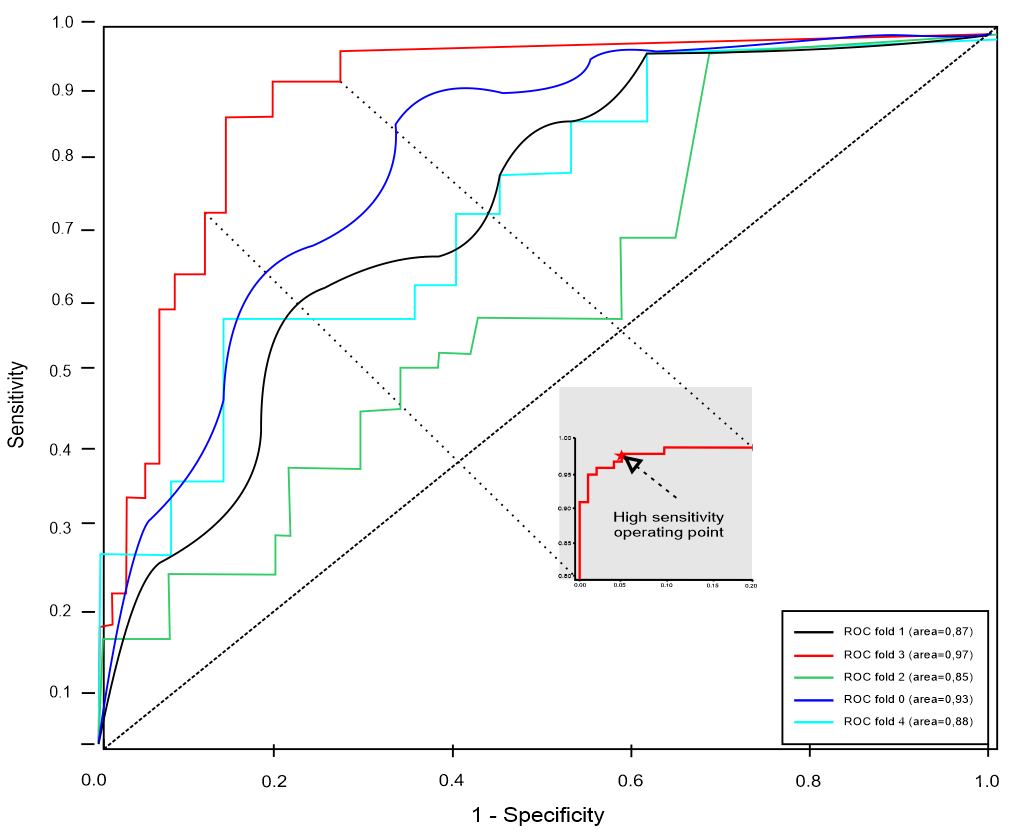
\includegraphics[width=0.9\linewidth]{images/roc_er.png}
		\caption{ER status classification}
        \label{fig:er_roc}
	\end{subfigure}
	\begin{subfigure}{.49\linewidth}
		\centering
		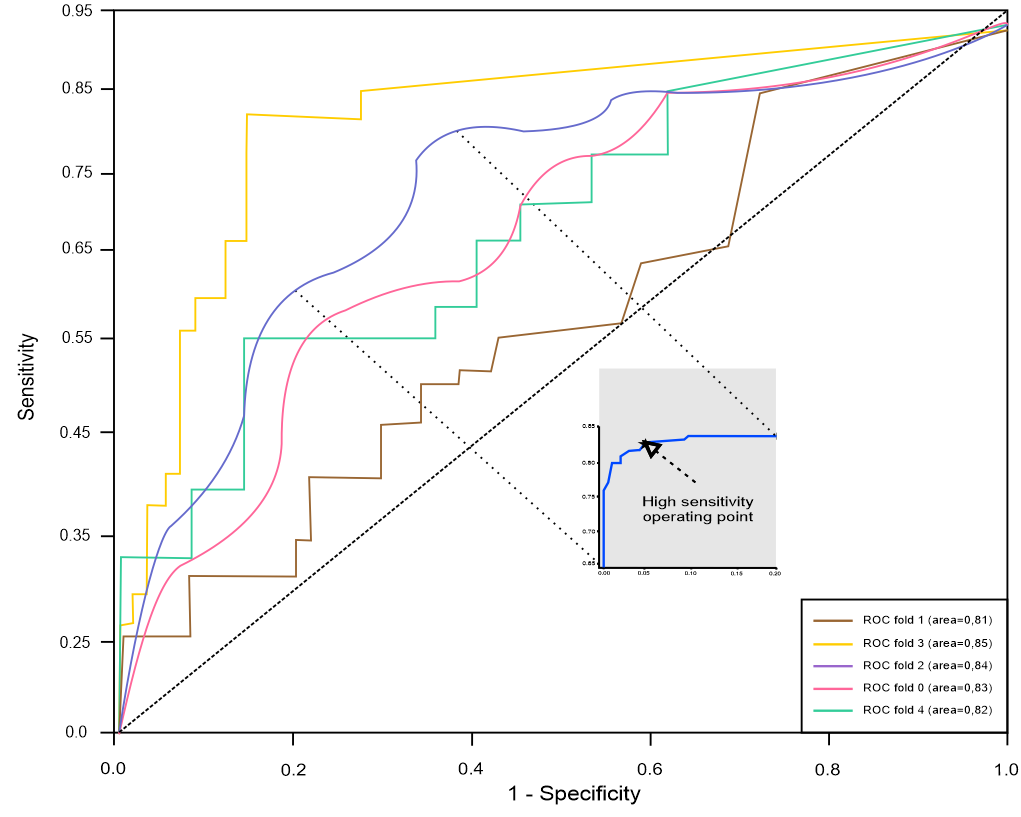
\includegraphics[width=0.9\linewidth]{images/roc_pgr.png}
		\caption{PGR status classification}
        \label{fig:pgr_roc}
	\end{subfigure}\\[1ex]
	\begin{subfigure}{0.49\linewidth}
		\centering
		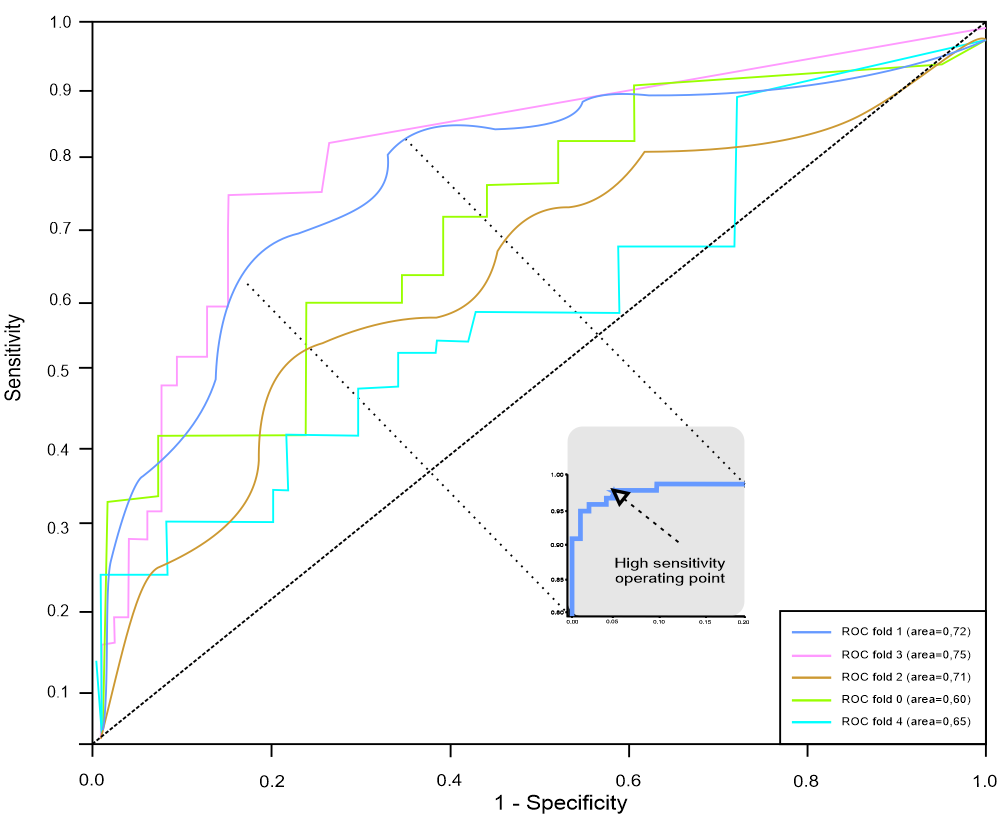
\includegraphics[width=0.9\linewidth]{images/roc_her2.png}
		\caption{HER2 status classification }
        \label{fig:her2_roc}
	\end{subfigure}
	\caption{ROC curve of the best predictor for ER, PGR, and HER2 status classification~\cite{karimACCESS2019}} 
	\label{fig:roc_all}
\end{sidewaysfigure*}

\subsection{Analysis of subtype classification}
The best results for ER status prediction are shown in in~\cref{tab:all_results} for each modality, where a combined input of GE and miRNA expression data performs the best than any single input modality. The confusion matrix in~\cref{fig:er_confusion} shows predictions about 288 breast cancer patients in which 197 were `ER Positive', 58 where `ER Negative', and 33 samples for `ER Indeterminate'. Out of 197 samples, the classifier classified 187 `ER Positive' cases correctly, making only 10 mistakes~(misclassification) in which 3 were misclassified as `ER Negative' and 7 of them were classified as `ER Indeterminate', giving overall high model confidence. 

\begin{table}[h]
    \centering
    \footnotesize
    \caption{Top results for ER, PGR, and HER2/neu status classification~\cite{karimACCESS2019}}
    \vspace{-2mm}
    \label{tab:all_results}
    \begin{tabular}{l|l|l|l|l|l} 
        \hline
        \textbf{Tasks} & \textbf{Input modality} & \textbf{MCC} & \textbf{Precision} & \textbf{Recall} & \textbf{F1} \\ 
        \hline
         & DNA methylation   & 0.7573 & 0.8948    & 0.8969 & 0.8958  \\ 
        \cline{2-6}
            & Gene expression  & 0.7745 & 0.8944    & 0.9004 & 0.8964  \\ 
        \cline{2-6}
        ER status       & miRA expression & 0.7235 & 0.8846    & 0.8876 & 0.8857  \\ 
        \cline{2-6}
                      & Gene + miRNA expression  & 0.7928 & 0.9325    & 0.9336 & 0.932   \\ 
        \cline{2-6}
                   & Gene + miRNA expression + DNA methylation & 0.7876 & 0.9175    & 0.918  & 0.9177  \\ 
        \hline
                     & DNA methylation   & 0.6963 & 0.7849    & 0.7939 & 0.7877  \\ 
        \cline{2-6}
                       & Gene expression  & 0.7134 & 0.8166    & 0.8276 & 0.8174  \\ 
        \cline{2-6}
        PGR status  & miRA expression   & 0.7059 & 0.7717    & 0.7743 & 0.7672  \\ 
        \cline{2-6}
                     & Gene + miRNA expression   & 0.7456 & 0.8566    & 0.8633 & 0.856   \\ 
        \cline{2-6}
                     & Gene + miRNA expression + DNA methylation & 0.7791 & 0.7987    & 0.8086 & 0.8001  \\ 
        \hline
                    & DNA methylation   & 0.5632 & 0.376     & 0.613  & 0.466   \\ 
        \cline{2-6}
                     & Gene expression   & 0.5967 & 0.6355    & 0.607  & 0.6173  \\ 
        \cline{2-6}
        HER2/neu status & miRA expression  & 0.6124 & 0.5627    & 0.5885 & 0.5732  \\ 
        \cline{2-6}
                   & Gene + miRNA expression   & 0.6276 & 0.6207    & 0.6444 & 0.627   \\ 
        \cline{2-6}
                   & Gene + miRNA expression + DNA methylation & 0.5743 & 0.3368    & 0.5804 & 0.4263  \\
        \hline
    \end{tabular}
    \vspace{-2mm}
\end{table}

\hspace*{3.5mm} Furthermore, as shown in the ROC curve in~\cref{fig:er_roc}, AUC scores for class 0, 1, and 2 are 0.91, 0.89, and 0.94, respectively, albeit we had only a few `Indeterminate' samples in the test set. The best results of PGR status prediction for each type of input is shown in~\cref{tab:all_results}. Similar to ER status prediction task, the predictor performs the best with the input of GE data combined with miRNA expression data. The other predictor with combined input of DNA methylation + gene expression + miRNA expression also performs relatively well. Best results are highlighted in green in~\cref{tab:all_results}. As seen from the confusion matrix in~\cref{fig:pgr_confusion}, the model is evaluated on 263 samples in which 167 were `PGR Positive', 75 `PGR Negative', and only 21 `PGR Indeterminate'. The best result was observed with the GE + miRNA expression input modality. As seen from~\cref{fig:pgr_roc}, AUC score for class 0~(`PGR Positive') and class 1~(`PGR Negative') are both 0.79, while 0.86 for class 2~(`PGR Indeterminate').

\begin{figure*}[h]
	\centering
	\begin{subfigure}{.49\linewidth}
		\centering
		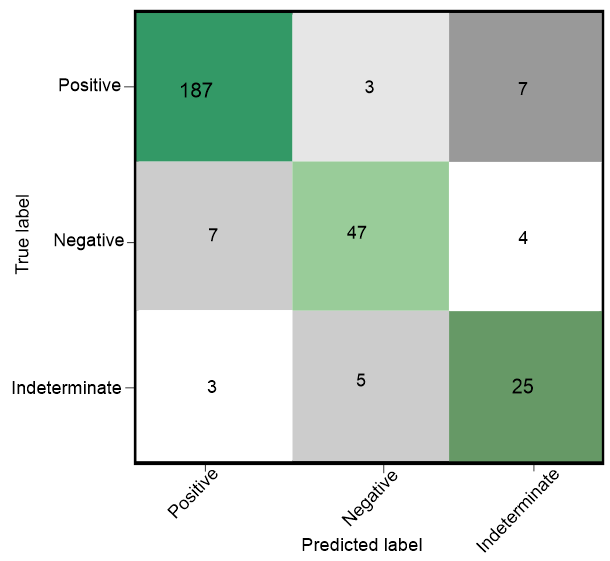
\includegraphics[width=0.85\linewidth,height=45mm]{images/conf_er.png}
		\caption{ER status classification}
        \label{fig:er_confusion}
	\end{subfigure}
	\begin{subfigure}{.49\linewidth}
		\centering
		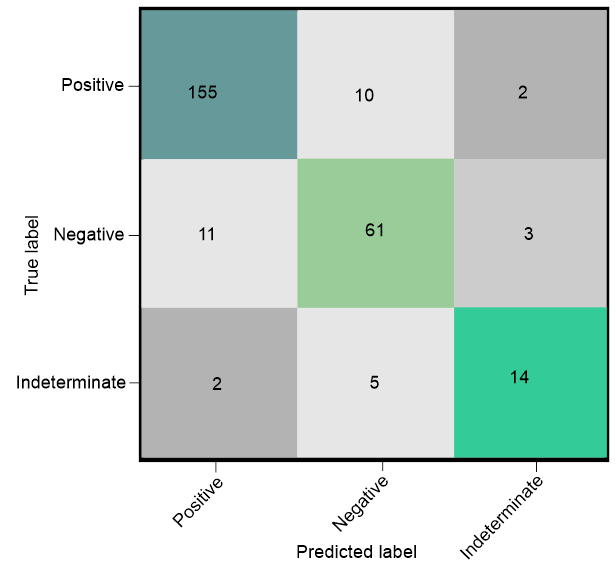
\includegraphics[width=0.85\linewidth,height=45mm]{images/conf_pgr.png}
		\caption{PGR status classification}
        \label{fig:pgr_confusion}
	\end{subfigure}\\[1ex]
	\begin{subfigure}{0.49\linewidth}
		\centering
		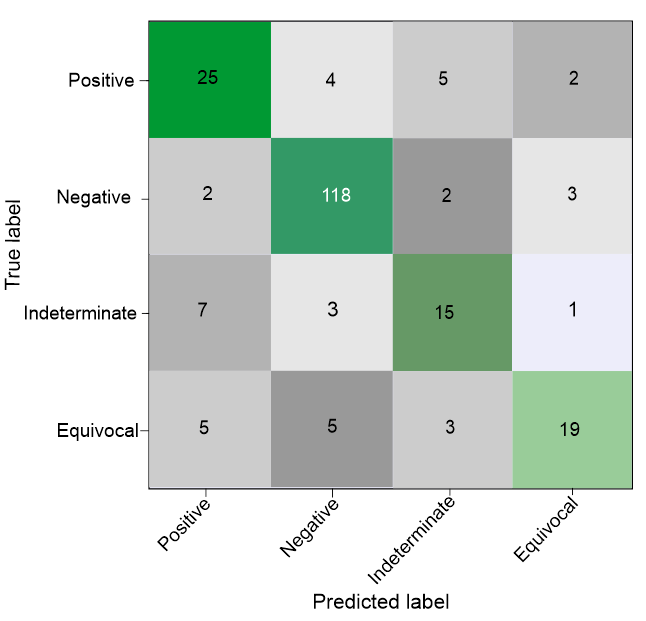
\includegraphics[width=0.85\linewidth,height=45mm]{images/conf_her2.png}
		\caption{HER2 status classification }
        \label{fig:her2_confusion}
	\end{subfigure}
	\caption{Confusion matrix for ER, PGR and HER2 status classification~\cite{karimACCESS2019}} 
	\label{fig:multi_cms}
\end{figure*}

%\subsubsection{Breast cancer subtype classification (HER2/neu status)}
\hspace*{3.5mm} The best results for HER2/neu status prediction for each type of input is shown in \cref{tab:all_results}. Similar to the ER and PGR status prediction tasks, the predictor performs the best with the input of GE data combined with miRNA expression data.  However, we observed overall a low accuracy score for each type of data, although, the performance on the training set itself was near to perfect. Even after applying several regularization techniques such as l2-regularization and Gaussian dropout layers, the result is still poor, which might be because of the overfitting. One of the possible causes for such overfitting is the smaller number of samples~(i.e. 860 samples) compared to ER and PGR statuses~(i.e. 1,024 samples).

\begin{figure*}
	\centering
	\begin{subfigure}{.49\linewidth}
		\centering
		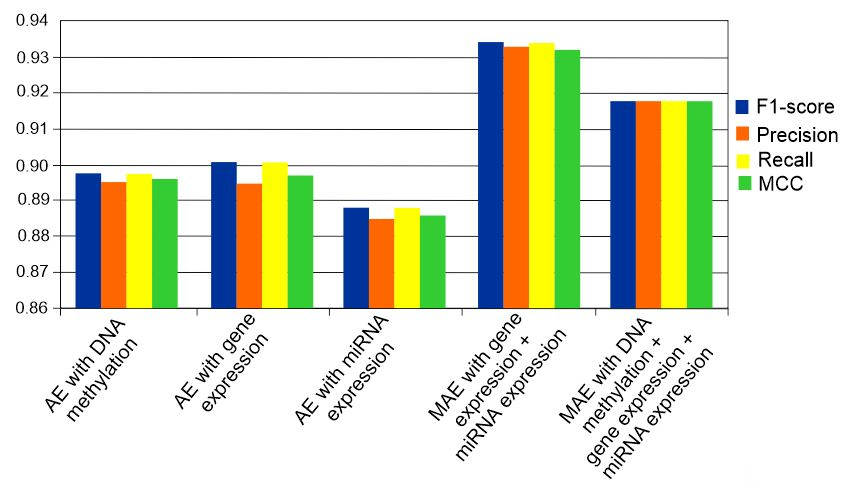
\includegraphics[width=0.8\linewidth,height=40mm]{images/1.png}
		\caption{ER status classification}
        \label{fig:top_er}
	\end{subfigure}
	\begin{subfigure}{.49\linewidth}
		\centering
		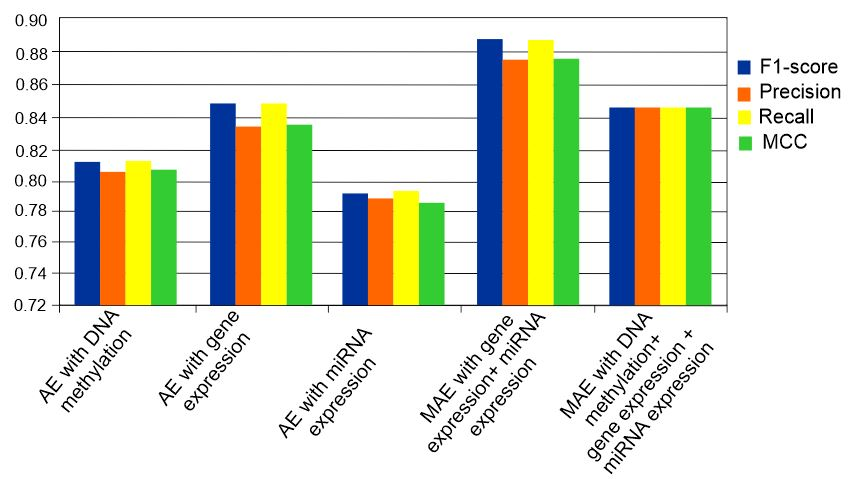
\includegraphics[width=0.8\linewidth,height=40mm]{images/2.png}
		\caption{PGR status classification}
        \label{fig:top_pgr}
	\end{subfigure}
	\begin{subfigure}{0.49\linewidth}
		\centering
		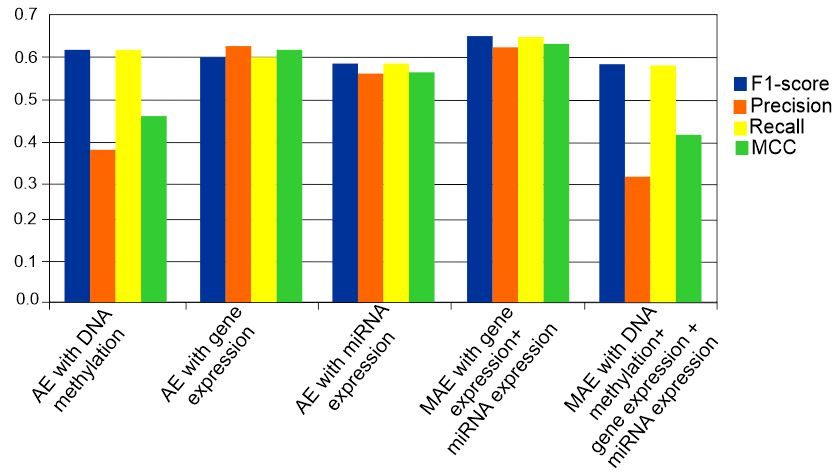
\includegraphics[width=0.8\linewidth,height=40mm]{images/3.png}
		\caption{HER2 status classification }
        \label{fig:top_her2}
	\end{subfigure}
	\caption{Top ER, PGR, and HER2 status classifications results for each input type~\cite{karimACCESS2019}} 
	\label{fig6}
		\vspace{-2mm} 
\end{figure*}

\begin{figure*}[h]
	\centering
	\begin{subfigure}{.48\linewidth}
		\centering
		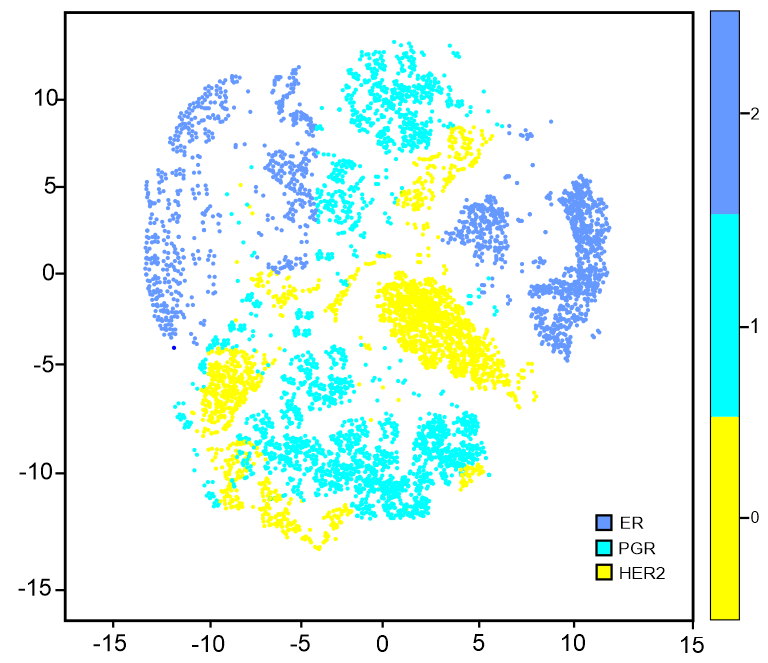
\includegraphics[width=0.8\linewidth,height=45mm]{images/raw_tsne.png}
		\caption{t-SNE plot of raw gene expression}
        \label{fig:tsne_raw}
	\end{subfigure}
	\begin{subfigure}{0.48\linewidth}
		\centering
		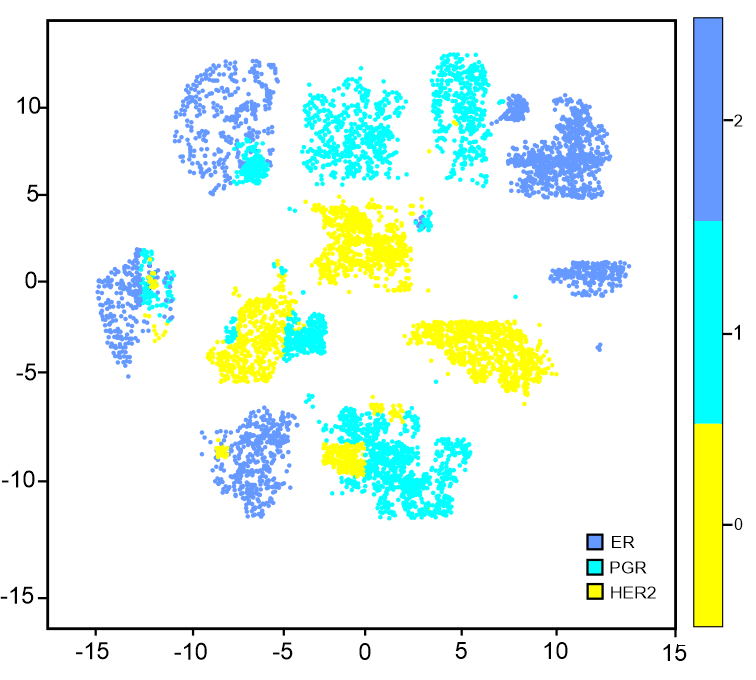
\includegraphics[width=0.8\linewidth,height=45mm]{images/ae_tsne.png}
		\caption{t-SNE plot of encoder's latent feature}
        \label{fig:tsne_ae}
	\end{subfigure}
	 \setlength{\belowcaptionskip}{-8pt}
	\caption{t-SNE visualization of gene expressions vs autoencoder latent feature map~\cite{karimACCESS2019}} 
	\label{fig:tnse}
	%\vspace{-2mm}
\end{figure*}

\hspace*{3.5mm} The best result based on gene + miRNA expression modality is highlighted in green in~\cref{tab:all_results}, while the corresponding confusion matrix is shown in~\cref{fig:her2_confusion}. As seen, the predictor is evaluated on 225 samples, with 40 of them actually `HER2/neu Positive', 121 of them are `HER2/neu Negative', 21 of them are `HER2/neu Indeterminate', and 32 of them are `HER2/neu Equivocal' in this test set. The classifier correctly predicted 173 `HER2' cases, making 48 mistakes showing overall low confidence giving about 80\% accuracy. Furthermore, the ROC curve of this experiment is shown in~\cref{fig:her2_roc}. As observed, with 2 out of 4 classes achieve lower than 0.5 AUC score: the AUC score for class 0 (`HER2/neu Positive') is 0.83, for class 1 (`HER2/neu Negative') is 0.73, for class 2~(`HER2/neu Indeterminate') is 0.36, and for class 3~(`HER2/neu Indeterminate') is 0.48. 

\hspace*{3.5mm} Further, inspired from literature~\cite{rhee2017hybrid} and to qualitatively study whether the learned representation can express biological characteristics of the patients, t-SNE of the MAE encoder's output i.e. latent feature map and the t-SNE plot with raw GE are plotted in \cref{fig:tnse}. We can observe moderately high distinctive patterns between three subtype patients. Since, all the input modality has high dimension, we consider the association between each feature. 

\iffalse
\subsection{Consistency of subtype prognosis}
Inspired from literature~\cite{rhee2017hybrid} and to qualitatively study whether the learned representation can express biological characteristics of the patients, t-SNE of the MAE encoder's output i.e. latent feature map and the t-SNE plot with raw GE are plotted in \cref{fig:tnse}. We can observe moderately high distinctive patterns between three subtype patients. Since, all the input modality has high dimension, we consider the association between each feature. 

\begin{figure*}[h]
	\centering
	\begin{subfigure}{.48\linewidth}
		\centering
		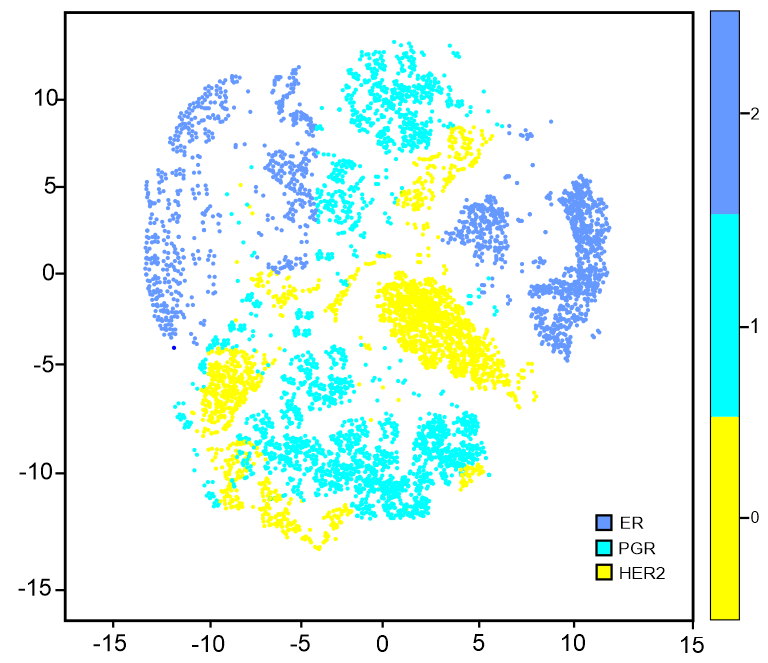
\includegraphics[width=0.9\linewidth,height=55mm]{images/raw_tsne.png}
		\caption{t-SNE plot of raw gene expression}
        \label{fig:tsne_raw}
	\end{subfigure}
	\begin{subfigure}{0.48\linewidth}
		\centering
		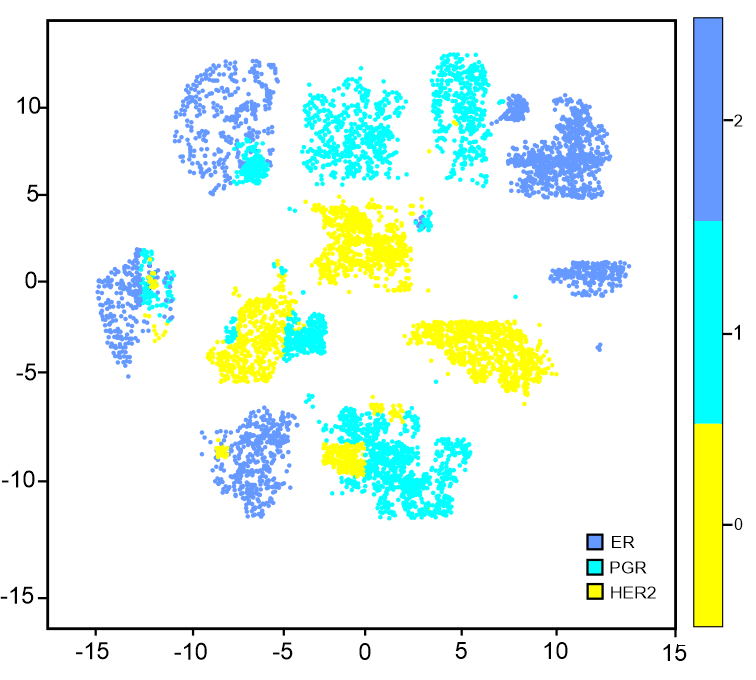
\includegraphics[width=0.9\linewidth,height=55mm]{images/ae_tsne.png}
		\caption{t-SNE plot of encoder's latent feature}
        \label{fig:tsne_ae}
	\end{subfigure}
	 \setlength{\belowcaptionskip}{-8pt}
	\caption{t-SNE visualization of gene expressions vs autoencoder latent feature map~\cite{karimACCESS2019}} 
	\label{fig:tnse}
\end{figure*}

\hspace*{3.5mm} Further, we can see that the order of subtypes in the t-SNE plot is identical to prognosis of breast cancer subtypes. Research~\cite{91Caruana} has exposed that 80\% of all breast cancers are `ER-positive' in which the cancer cells grow in response to the hormone estrogen. While about 65\% of these are also `PR-positive' in which the cancer cells grow in response to another hormone, progesterone. ER/PR-positive tumors are much more likely to respond to hormone therapy than tumors that are ER/PR-negative. In about 20\% of breast cancers, the cells make too much HER2 protein and tend to be aggressive and fast-growing\footnote{\url{https://www.webmd.com/breast-cancer/}}. In breast cancer, certain subtype has the worst prognosis e.g. basal, followed by HER2, Luminal B, and Luminal A. The reason is that basal subtype has distinctive molecular characteristics from other subtypes~\cite{bertucci2012basal}. However, not all these patterns clearly visible in the t-SNE plot with raw GE, which signifies that the MAE learned the latent molecular properties better from the patient expression profiles.

\subsection{Survival analysis}
\label{secExperimentationAndResults_ResRegression}
Similar to breast cancer subtype prediction, survival rate prediction task is performed with multi-type inputs. Best results for each type of input are shown in~\cref{tab:sur_results}, in which the overall lowest $MSE$ was recorded with the gene expression modality, although coefficient of the determination $R^2$ is negative. In case of DNA methylation + gene expression + miRNA expression modality, the MSE score is considerably high and the corresponding $R^2$ score is negative. These two cases indicates that the predictions are worse than the actual average output. In contrast, $R^2$ scores for the DNA methylation, miRNA expression, and gene expression + miRNA expression modalities are also positive, even though the corresponding MSE scores are lower than that of DNA methylation modality. Further, the $R^2$ is a positive value, which indicates it performs better than the actual average output. 

\begin{table}[h]
	\centering
	\caption{top results for survival rate prediction~\cite{karimACCESS2019}}
	\vspace{-3mm}
	\label{tab:sur_results}
	\begin{tabular}{l|c|c}
		\hline
		\multicolumn{1}{c|}{\textbf{Modality}}   & \textbf{MSE}  & \textbf{$R^2$}  \\ \hline
		DNA methylation & 0.26537  & 0.13054  \\ \hline
		Gene expression & {\color[HTML]{009901} 0.16541}  & -0.18753 \\ \hline
		miRNA expression & 0.34732 & 0.12468 \\ \hline
		\begin{tabular}[c]{@{}l@{}}Gene expression + miRNA expression\end{tabular}                     & {\color[HTML]{333333} 0.27615} & {\color[HTML]{009901} 0.19542}  \\ \hline
		\begin{tabular}[c]{@{}l@{}}DNA methylation + gene expression +\\ miRNA expression\end{tabular} & 0.57834 & -0.2735  \\ \hline
	\end{tabular}
\end{table}

\hspace*{3.5mm} To further evaluate the ability of the model to comprehend characteristics of molecular subtypes, we performed survival analysis inspired by literature~\cite{rhee2017hybrid}. We clustered the patients into two groups based on raw GE values and the MAE encoder's output i.e. latent feature map. K-means algorithm is used for the clustering and t-SNE is used for the dimension reduction and visualization. To the measure hazard ratios of different patient groups and to analyze the effectiveness of treatment by comparing the Kaplan-meier~(KM) plots (based on non-parametric statistics) of the treated and non-treated patient group are drawn for each of two clustering results as shown in~\cref{fig:km_sur_plot}.

\begin{figure*}[h]
	\centering
	\begin{subfigure}{.48\linewidth}
		\centering
		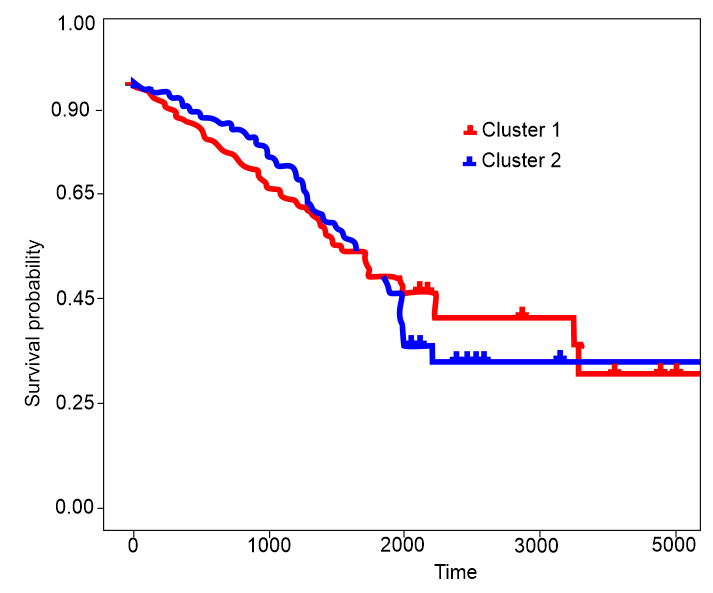
\includegraphics[width=\linewidth,height=60mm]{images/raw_cluster.png}
		\caption{KP plot of raw gene expression $p-value>0.05$}
        \label{fig:km1}
	\end{subfigure}
	\begin{subfigure}{0.48\linewidth}
		\centering
		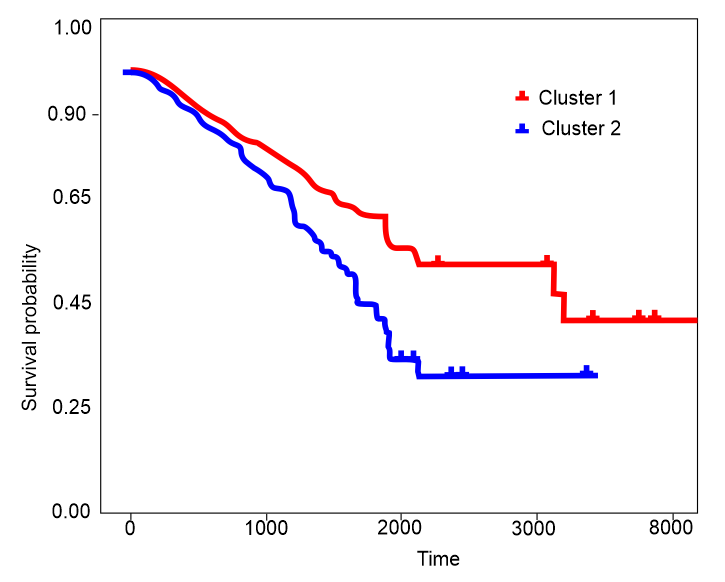
\includegraphics[width=\linewidth,height=60mm]{images/ae_cluster.png}
		\caption{KP plot of latent feature $p-value<0.05$}
        \label{fig:km2}
	\end{subfigure}
	\caption{Kaplan meier survival plots of the patients~\cite{karimACCESS2019}} 
	\label{fig:km_sur_plot}
\end{figure*}

\hspace*{3.5mm} The plot generated by the latent features~(\cref{fig:km2}) shows that the patient samples are more clearly separated into two subgroups showing distinct survival patterns with a $p-value<0.05$, while the plot with raw expression value~(\cref{fig:km1}) failed giving $p-value>0.05$. This is an interesting result as it shows that the model can simultaneously learn the genotypic information of patient from multimodal input features while performing the classification task.

\subsection{Comparison with ML baselines}
Although our datasets are collected from TCGA, multimodal features are used to train DL algorithms. Nevertheless, none of the related works summarized in~\cref{table:stateofart} used multimodality for breast cancer subtypes. 
%and survival prediction. 
Thus, a one-to-one comparison in a DL setting was not viable. Instead, we created unimodal and multimodal features out of each input type and train LR, KNN, NB, SVM, RF, and GBT as ML baseline models classifiers. 
%On the other hand, linear regression~($\hat{LR}$), Support Vector Regression~(SVR), Gradient Boosted Regression~(GBR), and random forest regression~(RFR) models were trained for predicting survival rates. 
In this setting, hyperparameters optimization is performed using random search with 5-fold cross validation. 

\hspace*{3.5mm} As shown in \cref{table:classification} 
%and \cref{table:regression}
, the GBT and RF-based classifiers 
%and regression models 
perform consistently best for subtype classification. %and survival prediction. 
The classification analysis can be further validated by calibrating the best performing MAE classifier against different embedding methods for which the output probability of the classifier can be directly interpreted as a confidence level in terms of `fraction of positives'~(FOP) as shown in~\cref{fig:cal}. As seen the MAE classifier gave a probability value~(i.e. FOP) between 0.82 to 0.93, which means 93\% predictions belong to true positives, whereas the second best GBT and RF generates the FOP values between 0.75 to 0.87 and between 0.76 to 0.89, respectively. 

\begin{table}[htp!]
	\renewcommand{\arraystretch}{0.9}
	\caption{survival prediction with ML regressors~(*=modality with best results)~\cite{karimACCESS2019}}
	\label{table:regression}
	\scriptsize
	\vspace{-2mm}
	\centering
	\begin{tabular}{p{2.8cm}|l|r|r}
		\toprule
		\textbf{Modality} & \textbf{Regressor} & \textbf{MSE} & \textbf{$R^2$} \\ \hline
		\multirow{4}{*}{DM} & $\hat{LR}$ & 0.4523 & -0.5432 \\
		& SVR & 0.6536 & -0.1156 \\
		& GBR & 0.3431 & -0.0135\\
		& RFR & 0.2314 & 0.0153\\
		\hline
		\multirow{4}{*}{GE} & $\hat{LR}$ & 0.6754 & -0.2348 \\
		& SVR & 0.5437 & -0.1102  \\
		& GBR & 0.2373 & -0.0653 \\
		& RFR & 0.1765 & 0.1176 \\
		\hline
		\multirow{4}{*}{miRNA} & $\hat{LR}$ & 0.8674 & -0.7832  \\
		& SVR & 0.6134 & -0.4569  \\
		& GBT & 0.5762 & -0.1542 \\
		& RF & 0.2956 & 0.1342\\
		\hline
		\multirow{4}{*}{GE+miRNA} & $\hat{LR}$ & 0.3451 & -0.1578  \\
		& SVR & 0.3538 & -0.3486  \\
		& GBR & 0.1937 & 0.0954 \\
		& RFR & 0.1456 & 0.1185 \\
		\hline
		\multirow{4}{*}{DM+GE+miRNA} & $\hat{LR}$ & 0.6523 & -0.8981 \\
		& SVR & 0.7287 & -0.7541  \\
		& GBR & 0.5123 & -0.6541 \\
		& RFR & 0.3287 & -0.2485 \\
        \hline
	\end{tabular}
\end{table}

\begin{figure}[htp!]
	\centering
	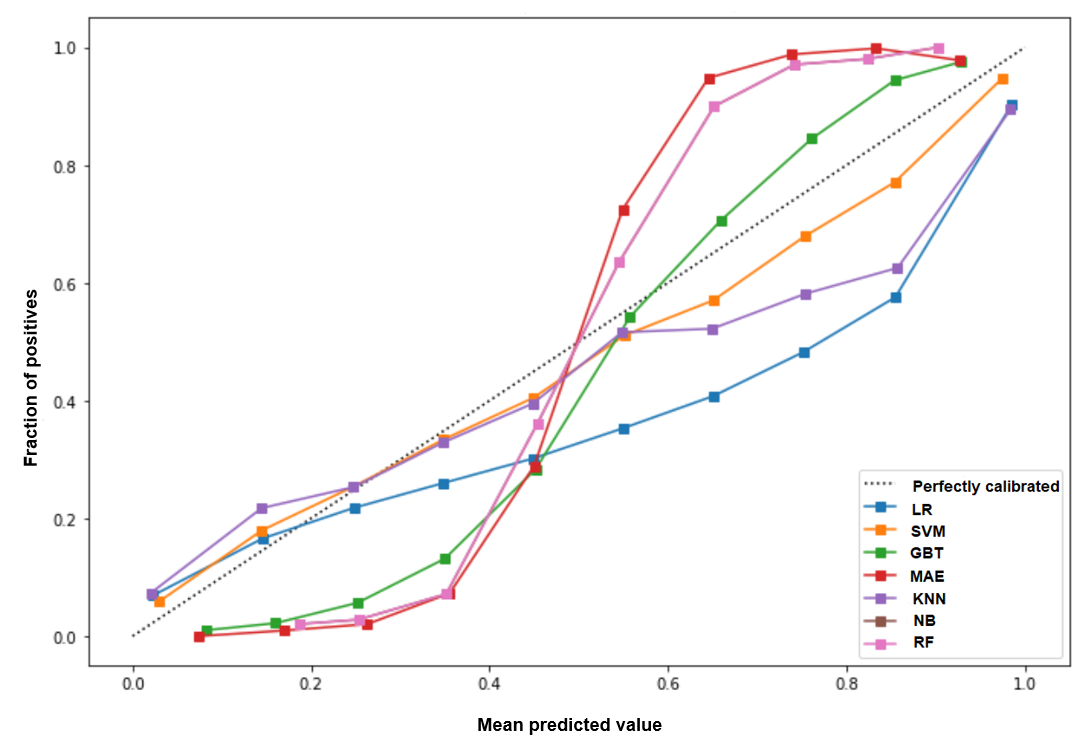
\includegraphics[width=0.8\linewidth]{images/cali.png}	
	\caption{Calibrating different classifiers~\cite{karimACCESS2019}}	
	\label{fig:cal}
\end{figure}

\begin{sidewaysfigure}[htp!]
	\centering
	\begin{subfigure}{0.48\linewidth}
		\centering
		\includegraphics[width=0.9\linewidth,height=80mm]{images/SVM.png}
%		\includegraphics[width=\linewidth,height=40mm]{SVM.png}
		\caption{SVM}
		\label{fig9a}
	\end{subfigure}
	\begin{subfigure}{0.48\linewidth}
		\centering
		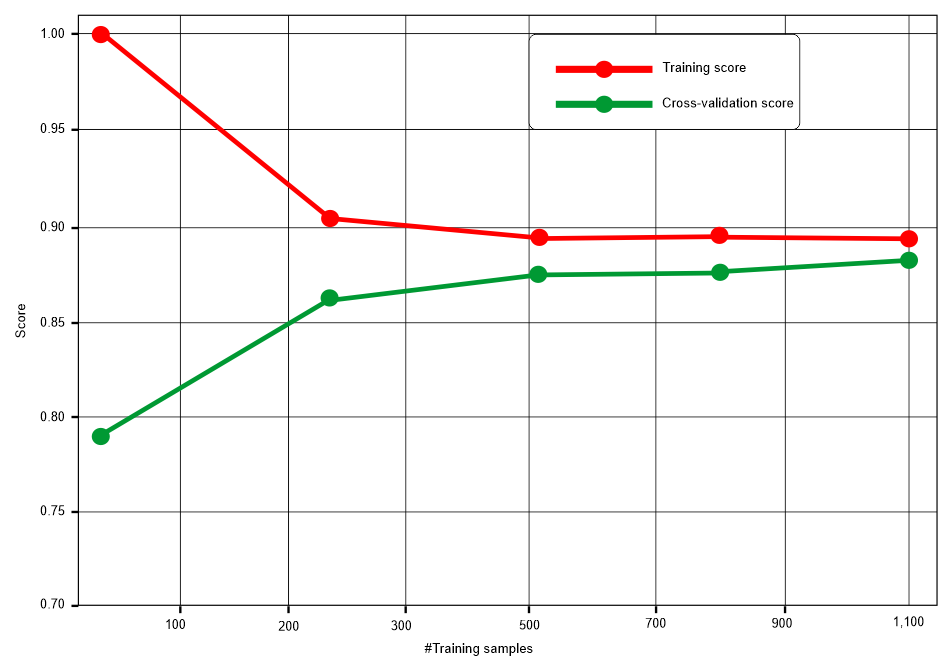
\includegraphics[width=0.9\linewidth]{images/GBT.png}
		\caption{GBT}
		\label{fig9b}
	\end{subfigure}
	\begin{subfigure}{0.48\linewidth}
		\centering
		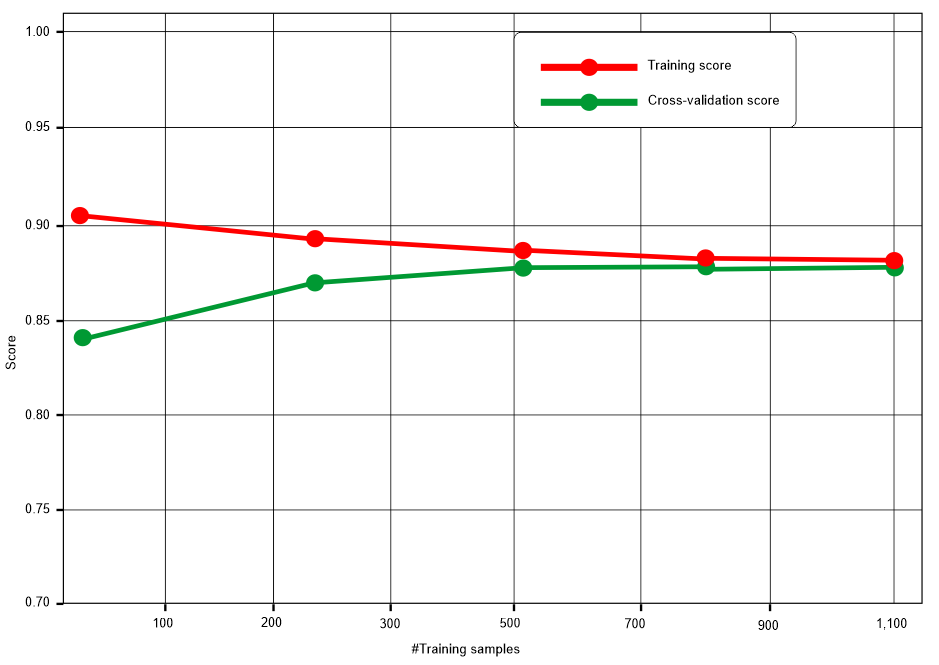
\includegraphics[width=0.9\linewidth]{images/RF.png}
		\caption{RF}
		\label{fig9c}
	\end{subfigure}
	\begin{subfigure}{0.48\linewidth}
		\centering
		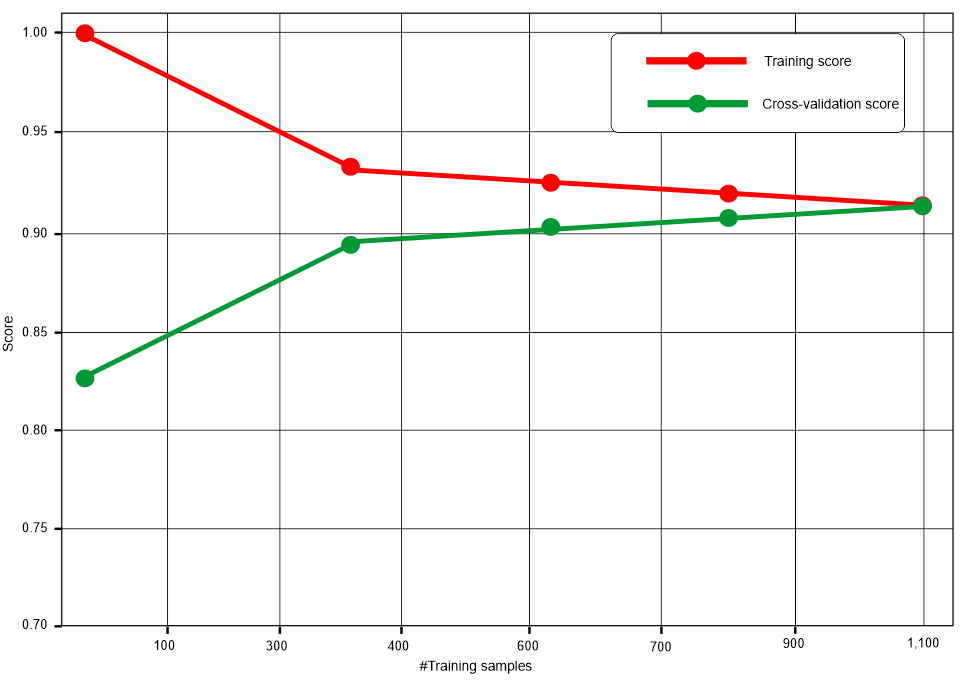
\includegraphics[width=0.9\linewidth]{images/MAE.png}
		\caption{MAE}
		\label{fig9d}
	\end{subfigure}
	\caption{Learning curves showing the validation and training scores of top-3 and SVM classifiers} 
	\label{fig:lc}
\end{sidewaysfigure}

\begin{table}
	\renewcommand{\arraystretch}{0.9}
	\caption{Subtypes prediction with ML classifiers~(*=modality with best results)~\cite{karimACCESS2019}}
	\label{table:classification}
	\vspace{-2mm}
	\scriptsize
	\centering
	\begin{tabular}{p{2.5cm}|l|r|r|r}
		\toprule
		\textbf{Modality} & \textbf{Classifier} & \textbf{Precision} & \textbf{Recall} & \textbf{MCC}\\ \hline
		\multirow{7}{*}{DM} & LR & 0.74 & 0.72 & 0.53 \\
		& NB & 0.73 & 0.70 & 0.55 \\
		& SVM & 0.80 & 0.81 & 0.69 \\
		& KNN & 0.69 & 0.71 & 0.51 \\
		& GBT & 0.88 & 0.85 & 0.72\\
		& RF & 0.91 & 0.92 & 0.75\\
		& \textbf{MAE}  & 0.93 & 0.91 & 0.79 \\
		\hline
		\multirow{7}{*}{GE} & LR & 0.76 & 0.72 & 0.59 \\
		& NB & 0.73 & 0.72 & 0.55 \\
		& SVM & 0.80 & 0.81 & 0.66 \\
		& KNN & 0.73 & 0.73 & 0.53 \\
		& GBT & 0.87 & 0.86 & 0.74\\
		& RF & 0.89 & 0.88 & 0.77\\
		& \textbf{MAE} & 0.92 & 0.91 & 0.79 \\ 
		\hline
		\multirow{7}{*}{miRNA} & LR & 0.75 & 0.73 & 0.54 \\
		& NB & 0.72 & 0.71 & 0.53 \\
		& SVM & 0.78 & 0.79 & 0.68 \\
		& KNN & 0.71 & 0.69 & 0.53 \\
		& GBT & 0.87 & 0.85 & 0.71\\
		& RF & 0.89 & 0.86 & 0.73\\
		& \textbf{MAE} & 0.89 & 0.90 & 0.75 \\ 
		\hline
		\multirow{7}{*}{GE+miRNA*} & LR & 0.72 & 0.71 & 0.57 \\
		& NB & 0.69 & 0.70 & 0.51 \\
		& SVM & 0.75 & 0.74 & 0.64 \\
		& KNN & 0.63 & 0.59 & 0.49 \\
		& GBT & 0.83 & 0.82 & 0.69\\
		& RF & 0.84 & 0.85 & 0.71\\
		& \textbf{MAE} & 0.87 & 0.88 & 0.74 \\ 
		\hline
		\multirow{7}{*}{DM+GE+miRNA} & LR & 0.65 & 0.68 & 0.47 \\
		& NB & 0.70 & 0.71 & 0.50 \\
		& SVM & 0.72 & 0.73 & 0.55 \\
		& KNN & 0.69 & 0.66 & 0.52 \\
		& GBT & 0.81 & 0.82 & 0.65\\
		& RF & 0.82 & 0.83 & 0.66\\
		& \textbf{MAE} & 0.84 & 0.85 & 0.69 \\
        \hline
	\end{tabular}
\end{table}

\hspace*{3.5mm} When it comes to survival prediction with ML regression models, the lowest $MSE$ was recorded with the gene expression modality using GBR regression model but much higher than that of MAE-based one. Whereas, the coefficient of determination $R^2$ is a positive value. In case of DNA methylation + gene expression + miRNA expression modality, the MSE score is considerably high and the corresponding $R^2$ score is also negative. These two cases indicates that the predictions are worse than the actual average output. On the other hand, $R^2$ scores for the miRNA expression, and gene expression + miRNA expression modalities are also positive but lower than that ones generated by MAE, even though the corresponding MSE scores are much higher than that of ones generated with MAE. In summary, the gene expression + miRNA expression modality shows the highest $R^2$  and lowest MSE score, which indicates it performs better than the actual average output showing moderately worse performance than that of MAE. 
\fi 

\subsection{Discussion}\label{chapter_4:discussion}
Overall the best results for breast cancer subtypes classification~(ER, PGR, and HER2 status) is generated from the MAE implementation with the input of GE and miRNA expression data, which is the best results for individual classification tasks. The HER2 status classification got the worst results by far compared to ER and PGR status ones, which is probably because the HER2 status data has fewer samples than ER and PGR ones. The training accuracy for each classifier far exceeds the test accuracy, probably because of overfitting. One reason is lack of training samples. As shown in~\cref{fig6}, the number of samples across datasets is only 1,000. While, the smallest number of feature~(e.g. 1,881 features in miRNA expression) still exceeds it, where the number of features in DNA methylation and GE exceeds other modalities. 
%In contrast, we experience varying results on survival prediction, e.g. AE achieves the lowest MSE score with the input of DNA methylation but giving a negative $R^2$ score, which means the prediction itself is not better than the average of the actual output. Positive $R^2$ scores were achieved with miRNA expression and GE + miRNA expression inputs using AE and MAE, respectively. To understand the effects of having more training samples, and to understand whether our classifiers suffer more from variance errors or bias errors, we observed the learning curves of top-3 classifiers~(i.e., RF, GBT, and MAE) and SVM~(a linear model) for varying numbers of training samples.

\hspace*{3.5mm} In our initial experiments, we observed by training ML models. For SVM the validation and training scores converge to a low value with increasing size of the training set. Consequently, SVM did not benefit much from more training samples. However, RF and GBT are tree-based ensemble methods, and the MAE model can learn more complex concepts from the GE + miRNA multimodal features. This results in a lower bias, which can be observed from higher training scores than the validation scores for the maximum number of samples i.e. adding more training samples does increase model generalization. Overall, MAE gave relatively better results compared to regular AE with a single type of input.
%as well as other best ML baselines, e.g., GBT and RF. 
It mostly occurs with the GE + miRNA expression giving the best results for subtypes classification.
%and decent results for survival rate prediction. 
Based on this comparison, we can conclude that there is a possibility MAE might surpass AE and ML baselines models such as GBT or RF performance with the right combination of inputs. 

\section{Chapter Summary}\label{chapter_4:conclusion}
In this paper, we developed a clin ical DSS, which is technically based on an MAE for predicting different subtypes of breast cancer patients.
%and their survival rates. 
Experiment results for the subtype classification are promising, especially based on the ER and PGR status having 0.93 F1-score, which produced with combined inputs of GE and miRNA expression data. 
%The performance result of the survival rate prediction shows varying signs. The best $MSE$ score is taken from predictors with DNA methylation as an input, although the $R^2$ score itself is negative, which indicate that it still performs worse than the simple average output. The GE + miRNA expression combination data as input gave very good results in general, although it did not have the best performance on the survival rate prediction.
However, the overall decision accuracy of DSS is hindered due to several factors: i) limited amount of labeled genomics data, which is probably individual patients privacy. This limitation causes of overfitting while training our neural network. 

\hspace*{3.5mm} The training scores is much higher than the validation scores for the maximum number of samples i.e. adding more training samples does increase model generalization. This suggest that the prediction can be made more confidently if we had more labelled training data, ii) secondly, we did not perform any feature selection but let the network to choose from the very high dimensional inputs. Consequently, for some input combinations the pretraining error for the MAE were getting out of bound, ii) limited amount of publicly available genomics data sources because other sources such as ICGC and COSMIC are not comprehensive even requiring restricted access. The DSS based on multimodal data is black-box, hence lack of interpretability. However, interpretability is important to gain insights into the reasons why a given cancer case is of a certain type can help in finding more accurate treatments and drug repositioning. Further, the ``right to explanation'', of EU GDPR~\cite{kaminski2019right} gives patients the right to know why and how an algorithm makes a diagnosis decision. 
%In the future, we intend to develop a more robust multimodal network such as multimodal Convolutional-LSTM to act both feature extractor and classifier and train with an enriched number of samples from other sources to develop an explainable deep architecture might open future opportunity to learn more towards potential gene set biomarkers based diagnosis. 

\hspace*{3.5mm} In the next chapter, we extend both single and multimodality-based cancer typing methods to overcome both limitations. We increase the number of samples, by combining samples from the PanCancerAtlas. We will focus on improving the explanations of the predictions using both ante-hoc approach by seeding explainability into the model from the beginning, to learn more towards potential gene set biomarkers based diagnosis. Further, to identify significant biomarkers, we will generate class-specific heat maps using guided-gradient class activation maps++~(Grad-CAM++) and layer-wise relevance propagation~(LRP). We will compute feature importance in terms of mean absolute impact, followed by ranking top genes across all the cancer types. Finally, we will provide explanations of the predictions.  
%In particular, we will focus on multimodality with reversed time attention model and Bayesian deep learning~\cite{choi2016retain}. 
